% TODO
% ----
% HOGG: One last pass to look at flow and citations 
% BOTH: Expand appendix B with the actual definition of the GI-Net model
% 

\documentclass[10pt]{article}
\usepackage[letterpaper]{geometry}
\usepackage{graphicx} % Required for inserting images
\usepackage{xcolor}
\usepackage{amsmath}
\usepackage{amsfonts}
\usepackage{amssymb}
\usepackage[title]{appendix}

% hogg layout / typesetting
\usepackage[framemethod=tikz]{mdframed}
\usetikzlibrary{shadows}
\definecolor{captiongray}{HTML}{555555}
\mdfsetup{%
  innertopmargin=2ex,
  innerbottommargin=1.8ex,
  linecolor=captiongray,
  linewidth=0.5pt,
  roundcorner=2pt,
  shadow=false,
}
\addtolength{\topmargin}{-0.25in}
\addtolength{\textheight}{1.50in}
\setlength{\headsep}{0.15in}
\setlength{\oddsidemargin}{0.30in}
\setlength{\textwidth}{5.90in}
\renewcommand{\paragraph}[1]{\smallskip\par\noindent\textbf{#1}~---}
\pagestyle{myheadings}
\markright{Hogg, Villar, \& Zanna / Improving emulators\hfill}
\setlength{\parindent}{1.4em}
\setlength{\textfloatsep}{0.00in}
\sloppy\sloppypar\frenchspacing

\begin{document}\thispagestyle{empty}
\section*{\raggedright
Using geometry and physics to improve machine learning emulators}

\textbf{David W. Hogg},\footnote{Center for Cosmology and Particle Physics, Department of Physics, New York University}
\noindent\textbf{Soledad Villar},\footnote{Department of Applied Mathematics and Statistics, Johns Hopkins University}
\&
\textbf{Laure Zanna}\footnote{Department of Mathematics, Courant Institute, New York University}

\medskip\noindent
\textit{A white paper submitted in 2023 September to ONR Applied and Computational Analysis}

\bigskip

\paragraph{Abstract}
In most of the physical science and engineering disciplines---and especially in multi-phase and multi-physics problems---the principal theories are computational:
They generate predictions or explanations for data via expensive simulations.
The computational load required for many important simulation-based projects exceeds the total scientific computing capacity of the United States.
Thus many projects are placing big bets on \emph{emulation}, in which an expensive simulation is replaced or augmented by a machine-learning model that is trained to replicate some aspects of the input--output relationship of the simulation, but at far lower computational cost.
Emulators have substantial limitations; the largest might be that it is hard to verify that the emulator is replicating the input--output relationship accurately; by construction full simulation-based verification isn't possible.
In this white paper, we describe two strategies that have the potential to improve trust in emulation.
In one strategy, we will build machine-learning model components---network layers---that provably obey a set of classical-physics symmetries, many of which are related to geometry.
These components make use of vector and tensor fields in the same way that the theories of physics are written in terms of vectors and tensors.
In the other strategy, we will develop adversarial attack methodologies against emulators, based on symmetries and conservation laws, to ``red-team'' emulators used in critical tasks in scientific and engineering projects.
These adversarial methods can be used to validate models, identify weaknesses, test data augmentations and other strategies, and create new training strategies.
Along the way we will apply these tools to contemporary problems in cosmology, climate and ocean science, which are areas that depend critically on emulators for their near-term goals.

\section{Emulators}
In physical sciences and in engineering, theoretical predictions are computed by complex computer simulations.
These have the property that they can deal with complex boundary conditions, and integrate nonlinear coupled equations.
Simulation cost is driven by the dimensionality of the problem, nonlinearities in the equations, and the range of scales (ratio of largest to smallest scale).
In most domains, it is impossible to simulate the full observable range of scales, at the accuracy desired for precision measurement and prediction.
Simulations are necessarily run in a trade space between accuracy and computational cost; anything that speeds simulations without sacrificing resolution delivers more science from current projects.
Now that Moore's Law has come to an end, new scalings must come from algorithms and methods, not brute force.

\paragraph{Climate and ocean science}
Climate and climate change are studied through coupled simulations of the ocean and atmosphere.
The Geophysical Fluid Dynamics Laboratory (GFDL) of the National Oceanic and Atmospheric Administration produces datasets for which simulations of physical models are corrected or constrained with real observations \cite{obrien2004gfdl, rutledge2006nomads, delworth2020spear}. 
For instance, the CM2.6 has a resolution of 10 km for the ocean with 50 vertical levels and a sea ice model, and 50 km for the atmosphere. 
Even though it is necessary to have high-resolution models, especially for addressing certain climate problems \cite{jong2023increases, pascale2020increasing, zhou2019toward}, high-resolution modeling comes at a high computational cost. Consequently, high-resolution climate models are used in conjunction with other tools, including machine learning, that are more amenable to exploring long time scales or focus on incorporating comprehensive climate processes.

\paragraph{Cosmology}
Two of the largest cosmology projects right now are the ESA Euclid project to measure large-scale structure \cite{euclid} and the Simons Observatory project to measure the cosmic microwave background \cite{simonsobservatory}.
These projects are both simulation-limited, in the sense that the precise measurements that they will make depend on precise comparison of the data with multi-physics simulations representing the cosmological model.
That model is multi-physics: It has a purely gravitational component, in which small primordial fluctuations grow into the observed structure, and a ``baryonic'' component that involves gas cooling, star formation, and winds and feedback from supernovae and black-hole accretion.
With traditional computational methods, it is not possible to do sufficient simulations at the accuracy and size required to make measurements as precise as the data natively permit.
These projects must augment their simulation suites with ma\-chine-learn\-ing-gen\-er\-a\-ted emulations.
The emulators are regressions that are trained to learn the input--output relationship of a simulation (or parts of it), and can be used as \emph{far faster} replacements for those simulations.
In Appendix~\ref{app:emulators} we describe five qualitatively different kinds of emulators, all of which are in use in cosmology at the present day.

One can ask, in general: \emph{Why would any emulator ever work?}
Isn't integrating the differential equations underlying the simulation with a good integrator going to be better than any machine-learning method trained thereon?
One answer is that a good emulator might effectively be learning a very high-order integration scheme.
Higher-order schemes are faster and more accurate than lower-order schemes in many physics problems \cite{highorder}.
Another answer is that the initial conditions are not fully general for most simulations.
Integrators are expected to integrate \emph{any} equations, given \emph{any} initial conditions and \emph{any} boundary conditions.
But the initial conditions of the Universe are very special, as are the boundary conditions for any ocean-science problem.
Thus the machine-learning method can learn and capitalize on sparseness or problem structure generated by the restrictions on the problem setup.
Another answer is that sometimes only certain things are needed from the simulation; the simulation need not be accurate in all respects.
If the training loss is sensitive to this, the emulator can learn to emulate what it needs to.

\section{Trustworthiness of emulator outputs}

Emulators can enormously speed up computations.
That's because the emulator is not doing the same computation as the simulation it is replacing.
That opens up big scientific risks:
If an emulator is delivering inaccurate outputs, the scientific projects making use of those emulators are compromised.

There are some contexts in which the output of an emulator can be checked with full simulations.
For example, if the emulator is used to speed real-time triggers, the outputs of those triggers can often be checked \textsl{ex post facto} with full simulations.
However, in most applications in scientific domains, the scientific results that depend on the emulators cannot be fully checked by the running of full simulations.
This is because the emulators were built in the first place because full simulations are too expensive.
For example, in contemporary cosmology projects, large numbers of simulations are required in order to estimate the expectation value of the galaxy clustering (or power spectrum), and even more simulations are required in order to estimate the variance (covariance matrix) on that prediction.
The number of emulated simulations required for a project like the Simons Observatory is so large that it would be impossible to fully validate with full simulations.

Thus there is a trust issue with emulators:
How do we trust the results of a data analysis or prediction that is made with an emulator when we cannot afford to fully check it with a full suite of simulations?
Related to this, \emph{emulation brings significant risk of confirmation bias}:
Since verification of an emulation-based result is very expensive, the motivation to verify the result with full simulations will strongly depend on how surprising the community finds the result.

\textbf{In this white paper we recommend two strategies to improve the trustworthiness of emulators.}
These two strategies are not intended to comprehensively address or solve the trust issue with emulators, but they are intended to provide a start.
The first of these strategies is to bake in, at design time, geometric and physical symmetries at the machine-learning network level.
The second is what an engineer might call ``red team'' or adversarial attack, in which geometric and physics knowledge is used to design attacks that reveal (and fix) flaws.

\section{Enforcing classical symmetries}

Most simulations integrate equations by discretizing geometric objects onto lattices or grids.
These could be concentrations (scalars), velocities (vectors), magnetic fields (pseudovectors), or stresses (2-tensors) on a surface or in a volume.
These fields---or these discretized representations of fields---are \emph{geometric} in the sense that they are defined in terms of their transformation properties under geometric operators such as rotation, translation, and reflection.
Thus, there is a need for machine learning methods designed for geometric images—lattices or grids of scalars, vectors, and tensors.

In \cite{gregory2023geometricimagenet} we propose GeometricImageNet. We generalize the concept of convolution to geometric images such that the outputs of the convolutions are also geometric images, obeying the same geometric transformation rules as the inputs.
The fundamental observation that inspires this work is that when an arbitrary function is applied to the components of vectors and tensors, the geometric structure of these objects is destroyed. There are strict rules, dating back to the early days
of differential geometry \cite{ricci}, about how geometric objects can be combined to produce new geometric objects, consistent with coordinate freedom and transformation rules. These rules constitute a theme of Modern Classical Physics \cite{mcp}, where they are combined into a Geometric Principle. 

In a nutshell, in order to apply a CNN to a vector or tensor field without destroying the geometric structure, the convolutional filters need to be geometric objects themselves, acting by outer products.
Contractions expressed with Einstein summation notation can be applied to reduce the order of the geometric objects, for example, from tensor images to scalar images (or from tensor images to pseudovector images). See \cite{gregory2023geometricimagenet} for a precise definition of the GeometricImageNet model and Figure~\ref{fig.GINet} for an illustration. 
\begin{figure}[t!]\begin{mdframed}
    \centering
    \begin{minipage}{0.85\textwidth}
    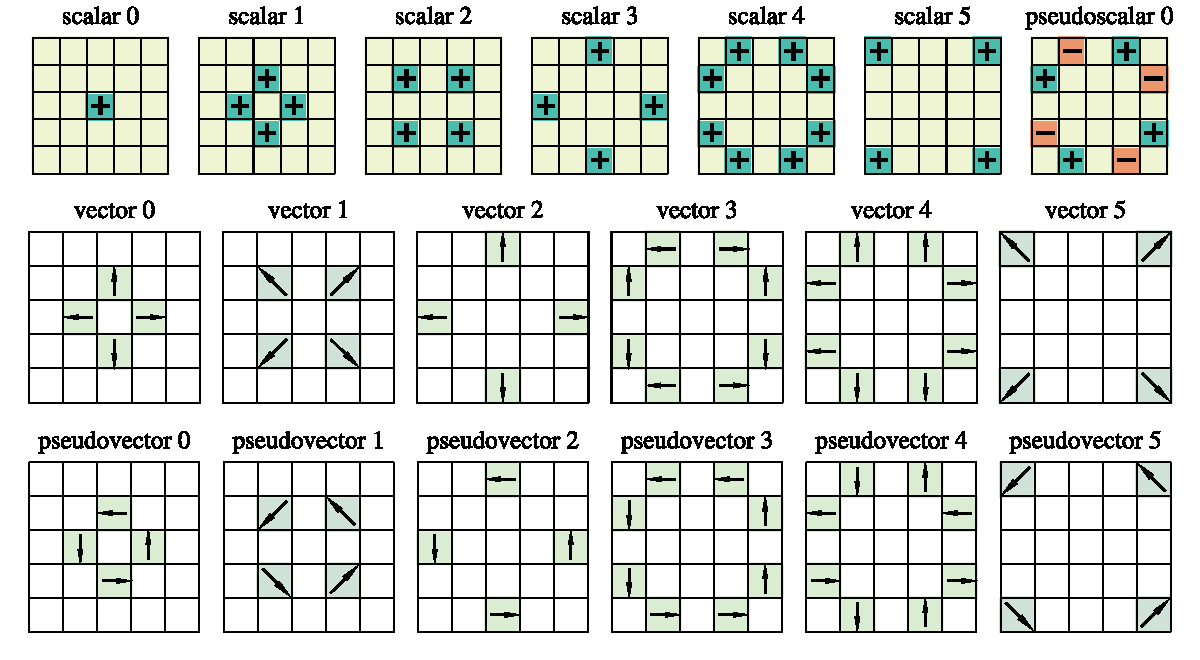
\includegraphics[width=\textwidth]{filters_m5.pdf}
    \end{minipage}
    
    \begin{minipage}{\textwidth}
    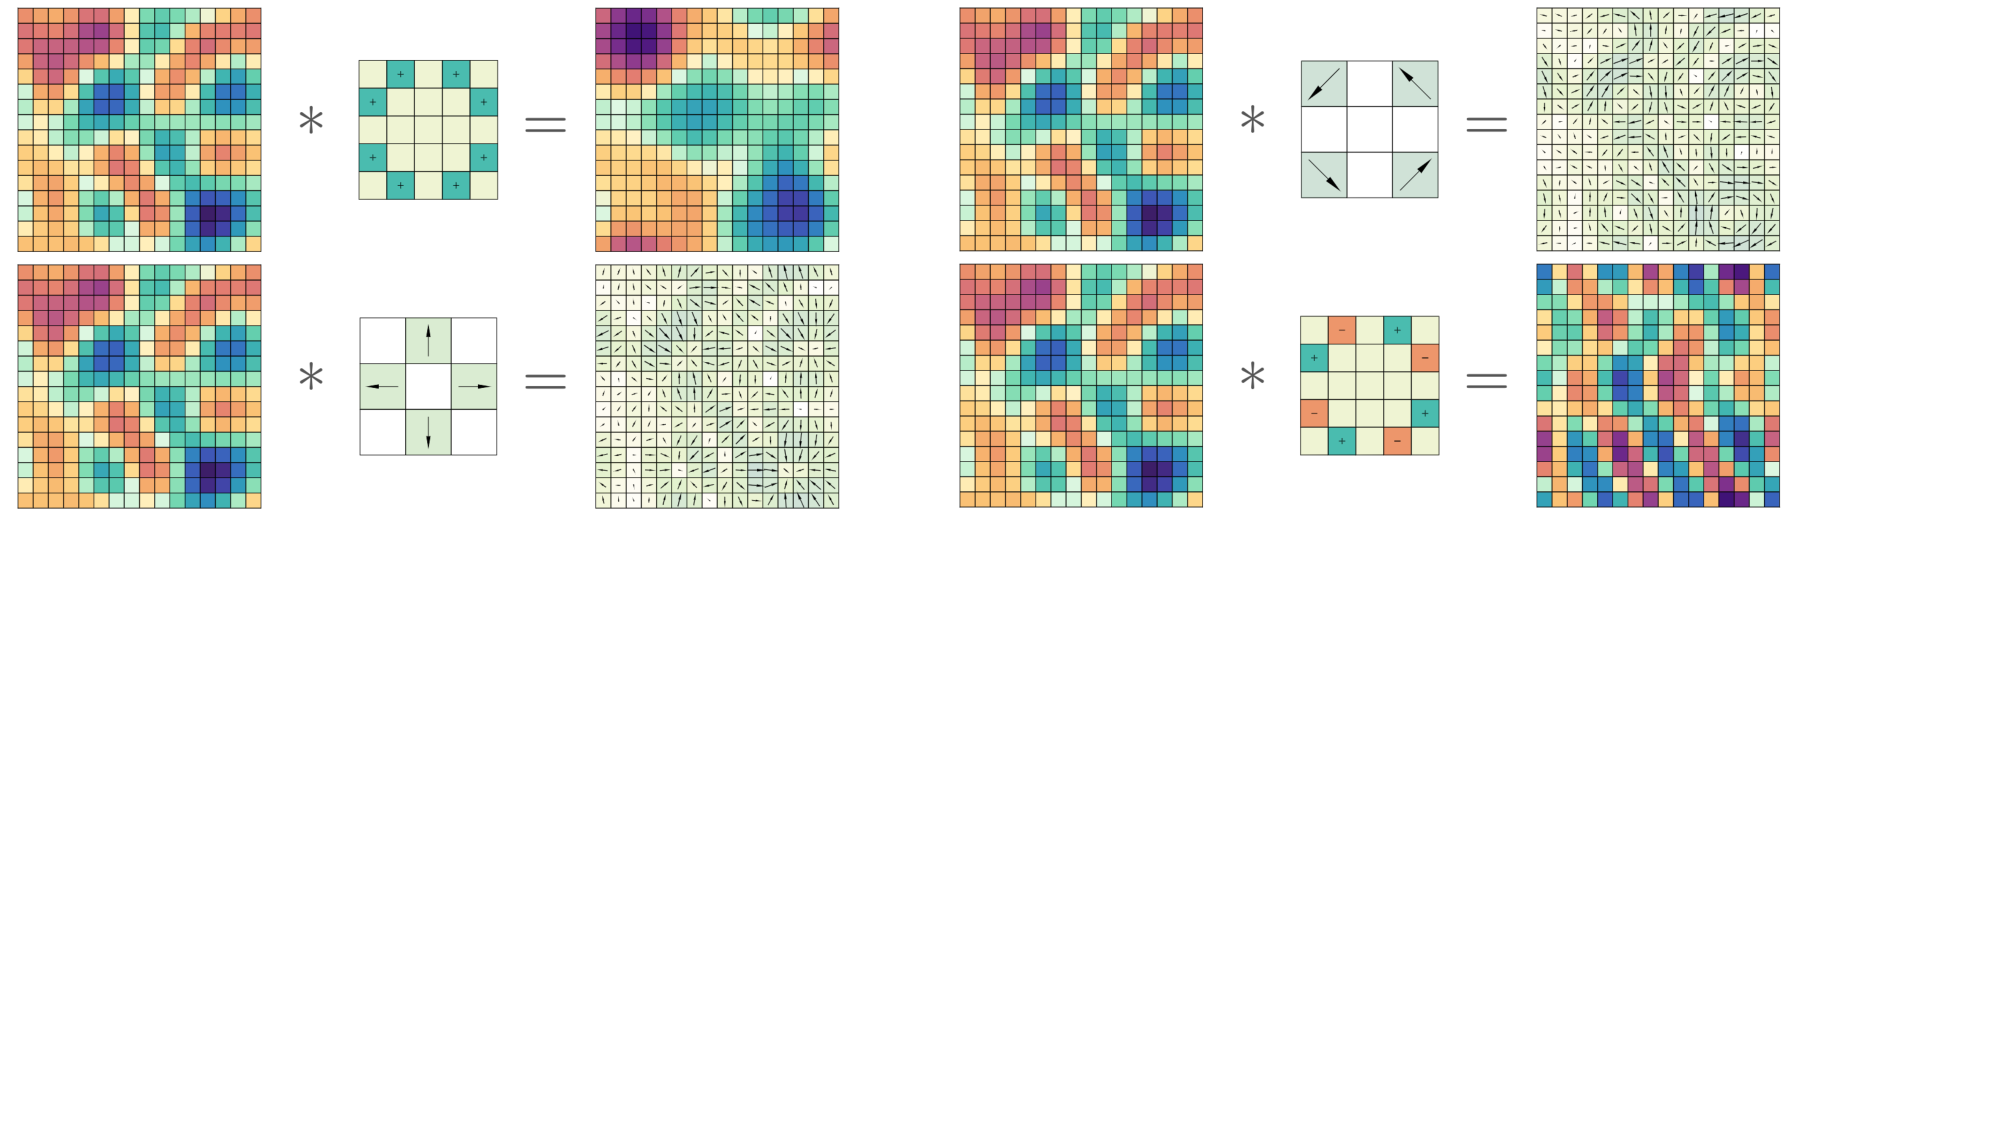
\includegraphics[width=\textwidth]{convs.pdf}
    \end{minipage}
    \vspace{-.3cm}
    \caption{(Left) The 5x5 scalar, pseudoscalar, vector, and pseudovector symmetric filters for 2-D images. (Right) Convolution of a scalar image with different geometric filters. Note the convolution with a scalar filter can be seen as the discretization of a diffusion operator, and the convolution with the vector filter resembles a discretization of the gradient. In general any symmetric discretization of any coordinate-free operator (gradient, divergence, curl) could be expressed in terms of our symmetric filters. Details for how these kinds of operations can be combined into a machine-learning network model are given in Appendix~\ref{app:architecture}.}
    \label{fig.GINet}
\end{mdframed}\end{figure}

Any symmetric discretization of any coordinate-free operator (gradient, divergence, curl) could be expressed in terms of our symmetric filters.
Therefore, this model is a natural tool to emulate the dynamics of physical models, arising from unknown (or partially known) PDEs, as done in the physics-informed machine learning literature \cite{karniadakis2021physics, hao2022physics}.
It is an alternative approach to the more general theoretical frameworks from \cite{steerable, jenner2021steerable, bhardwaj2023steerable, clifford} that is specifically tailored to work for geometric images.   

Sometimes square, image-like discretizations are used even when they aren't really appropriate.
An example is the ``tripolar grid'' used for ocean dynamics simulations and data representation.
This grid is square everywhere over the oceans, but different pixels have very different areas, depending on their distances rom the three poles of the tripolar grid.
The GeometricImageNet we have developed can be augmented with per-pixel 2-tensor metric information that will permit machine-learning methods to properly account for the fact that the square grid has been warped onto the intrinsically curved spherical surface of the oceans.

Finally, we remark that not all simulations and data are represented on grids of discrete points.
Indeed, in cosmology both simulations and data are often represented with spherical harmonics on the sky.
Spherical harmonics are one kind of useful basis function; simulation methods that work in the space of continuous basis functions are called spectral methods.
The tools we are building to represent grids or arrays of vectors and tensors can be generalized to continuous basis-function representations.
The vector spherical harmonics are known, and we have developed expressions for the higher-order tensor spherical harmonics, to any tensor order.
Thus everything that can be done with GeometricImageNet could be done also in a spherical-harmonic representation.
There are also possible generalizations for wavelets and other kinds of bases, which could be very useful for representing data and creating new kinds of neural networks to work on vector and tensor fields.

\paragraph{Emulation experiments: Cosmology}
Recent works in computational cosmology employ deep neural networks to enhance low-resolution dark matter-only simulations, generating super-resolution realizations that agree remarkably well with the full simulation counterparts on their statistical properties and are orders of magnitude faster \cite{li2021ai, ni2021ai}. 

In general, the n-body simulations are initialized on a cubic lattice, with the initial conditions encoded as small position and velocity displacements away from the perfect cubic lattice. Thus the points in the n-body simulation start on a regular grid, and can be identified throughout the simulation evolution with their initial grid locations.

For instance, in \cite{li2021ai} the evolution of the n-body simulation is represented with a 3D grid with 3 channels (each
channel corresponds to one component of the displacement vector). A deep learning model, based on StyleGAN2 \cite{karras2020analyzing}, takes the low resolution particle displacements as input, and outputs a possible realization of their high resolution counterparts. They use data augmentation to regularize the model to be approximately $SO(3)$-equivariant. 

We propose to improve emulators such as \cite{li2021ai, ni2021ai} by using a 3D geometric image to represent positions (and velocities) instead of a 3D grid with 3 (or 6) independent channels. The evolution equations are independent of orientation and position (they are coordinate free!), so they are implementable as a GeometricImageNet model. Current state-of-the-art on such emulators do not enforce any symmetries beyond simple translation symmetry or data augmentation; they do not enforce O(3) symmetry or Lorentz invariance or Hamiltonian phase-space-density conservation.

\paragraph{Emulation experiments: Ocean dynamics}
Climate and climate change are studied through multi-phase coupled simulations of the ocean and atmosphere.
For ocean dynamics, the primitive equations are derived from the Navier-Stokes equations on a sphere, considering the impact of Earth's rotation and complex boundary conditions.
Additional assumptions include the hydrostatic balance between the ocean and atmosphere, incompressibility of the fluid, and small temperature and density variations.
Under these assumptions, the resulting equations are in what is known as the Boussinesq approximation, where the fluid density remains constant, except for tiny variations accounted for with a buoyancy.
The resulting differential equations are of course independent of the coordinate system.

We propose GeometricImageNet as a tool with the right inductive bias to incorporate in the existing computational pipelines, as a replacement for CNNs in emulation tasks \cite{bolton2019applications}.
One standard emulation task is forecast:
Given the initial conditions, predict the state of the ocean $X$ days, months, or years into the future.
The scaling enabled by fast emulators permits the production of forecasts with uncertainties (or probabilistic forecasts).
Another standard task is parameter calibration:
The emulator is used to generate inexpensive long integrations with variations in simulation parameters (mixing coefficients, say) that are uncertain, but which only show the effects of those variations over decade timescales.
It is hard to calibrate these parameters without many simulations that extend for many decades.

\section{Symmetry-based adversarial attacks}

In deep learning, neural network classifiers have been shown to be extremely vulnerable to imperceptible perturbations to their inputs, which can cause the classifier to predict an erroneous output \cite{biggio2013evasion, szegedy2013intriguing, goodfellow2014explaining}. Examples of such adversarial attacks include the Fast Gradient Sign Method (FGSM)  \cite{goodfellow2014explaining} and the Projected Gradient Method (PGD) \cite{madry2017towards}, which produce small additive perturbations to the input that are bounded in $\ell_p$ norm and designed to maximize the loss of the classifier. A similar behavior can be obtained by perturbing the training set by poisoning \cite{shafahi2018poison, metzen2017detecting}.

In the setting where there may be bad actors, adversarial attacks are a critical issue, since these perturbations can cause significant security risks in deploying neural networks in real-world applications. In the emulation application we envision in this project we don't expect to have bad actors, but \textit{the existence of adversarial attacks show that the model is not computing what we expect}.
Mitigating unexpected and physically impossible modes is desirable.  

In response to adversarial attacks, many defense methods have been developed, including adversarial training \cite{kurakin2016adversarial} which augments the training set with adversarially generated examples, Defense-GAN \cite{samangouei2018defense} which projects the corrupted input onto a clean manifold, and Randomized Smoothing \cite{cohen2019certified} which selects the most likely label under Gaussian perturbations to the input.
However, such defenses have been broken by new attacks \cite{athalye2018synthesizing,athalye2018obfuscated, carlini2017adversarial, uesato2018adversarial, athalye2018robustness}, which have motivated new defenses \cite{madry2017towards, samangouei2018defense, zhang2019theoretically, papernot2016distillation, kurakin2016adversarial, miyato2018virtual, zheng2016improving}, and so on, leading to an arms race between new attacks and new defenses. %While stronger defenses with provable certificates of robustness continue to be developed  \cite{steinhardt2017certified,levine2019robustness}, a mathematical understanding of why deep networks can be fooled into making wrong predictions, or how to design and train networks with guarantees of robustness remains elusive. 

In this white paper we propose to extend the definitions and analysis of adversarial attacks to classical-physics contexts. The classical symmetries, including translation, rotation, boost, units covariance, particle permutations, and so on, lead to very precise predictions for simulation outputs given simple transformations of simulation inputs.
Thus, these symmetries guide novel physics-informed adversarial attacks.
In addition, there are associated conservation laws in many cases, such as energy, angular momentum, linear momentum, mass, and so on.
All of these symmetries are in play in a passive sense in almost all natural-science and engineering problems: The underlying laws of physics obey all these symmetries exactly.
That said, most of them are broken an active sense: The boundary conditions, initial conditions, and problem contexts break the passive symmetries so they don't always appear actively in the input--output relationship of the simulations.
In Appendix~\ref{app:adversarial} we describe a few possible adversarial attacks that are designed to evaluate the robustness of the model at complying with physical law. However, designing physics-based adversarial attacks and adversarial training against those attacks is a primary thrust of the proposed research. 

Since simulators are defined in terms of the physics, we expect them to be robust to physics-based attacks (though they may be vulnerable to attacks that get at discretization, numerical stability, or approximations).
Emulators, however, are deep learning models that typically are not designed specifically to obey any particular physics.
In the previous section we proposed an approach to enforcing certain symmetries arising from physics in the design of the machine learning model.
However, it is not known how to impose all symmetries and conservation laws in play. Here we propose an alternative approach. We propose to define adversarial attacks to the physical symmetries, and to design adversarial training methods to produce models that approximately satisfy physical constraints robustly.
We propose to compare this approach to data augmentation, however, we expect the new approach to be significantly more robust.

%MAIN POINT: simulators are robust to physics (we hope). Emulators are probably not since they are based on deep learning (and maybe protected via data augmentation if lucky). Our goal is to make the emulators do something physically reasonable. If we can attack on this then the emulator is wrong. We propose to make emulators that are robust to phyiscs attacks (for now we consider conservation laws and symmetries but we expect to find more in this research, figure out more). Some phyisics we can incorporate using the things described above. But other things like conservation laws are not known how to impose them in a close form. We do it by building an attack and adversarially trained. So questions we want to answer: 
%is this better than data augmentation?
%how robust are both the simulators and emulators?
%develop new possible attacks to the physics
%design adversarial training for symmetry-based and conservation-based and deploy it in cosmology and ocean science.
%evaluate how well this works. 


%How would red-team attacks help an emulator?
%The simplest answer is that they would provide a new set of tests for the emulator, going beyond simple performance on held-out training data (validation or test data).
%Held-out data can rarely span the range of conditions in which an emulator is expected to perform well, so any additional validations are valuable.
%The next answer is that successful attacks reveal emulator flaws, which can be subsequently removed or trained out.
%A successful attack suggests that either the emulator needs to be structured to have less capacity in symmetry-violating parts of function space, or else that the emulator needs much more training data.
%Indeed, many symmetries are currently enforced by data augmentation techniques (SOLE CITATIONS); symmetry-based attacks could be used to set the magnitude of the augmentation.
%The next answer is that once attacks have been designed, they can be incorporated into the cost function or training of the emulator, to ensure that future training rounds will deliver emulators that are not susceptible to those attacks.
%Of course it is an ``arms race'' in the sense that as attacks improve, emulators will have to improve to defend against them.

%Not all emulators are equally susceptible to attack, for many reasons.
%The most susceptible will be those that attempt to generate large, complex simulation outputs.
%For example, in a cosmological n-body simulation with $10^{10}$ particles, there are literally billions of nuisance parameters---phases of the random draw for the initial conditions---and thus it would be impossible for an emulator to be trained on truly representative data that span this initial-conditions space.
%Emulators in this context will be very susceptible to attacks.
%In contrast, emulators that produce only a few numbers (statistics say) that summarize the simulation outputs, they end up being more like interpolators than emulators, and will not have nearly as much susceptibility to attack.

\clearpage\begin{appendices}
\section{The types of emulators}\label{app:emulators}
There are five different kinds of emulators in use in the physics domains with which we interact:

\paragraph{Full replacement}
The most extreme---and most standard---kind of emulator is one that simply replaces the full input--output relationship of the entire simulation.
Thus if the simulation starts with initial conditions and boundary conditions, and ends with a final state (after an integration), the full-replacement emulator would be trained to learn the full relationship between the initial and boundary conditions and the final state.
A full-replacement emulator is a complete, plug-in replacement for the simulator.

\paragraph{Integrator}
Simulation run times generally scale linearly with the number of time steps required to execute the integration.
A set of emulators can be trained on a set of snapshots of the simulation internal state at a set of times that is much smaller than the full set of integration time steps.
Each emulator is trained to learn the relationship between the internal state of the simulation at one time $t_A$ and the internal state of the simulation at a later time $t_B$, such that the emulator can be used to replace the integrator during the time interval from $t_A$ to $t_B$.
A set of such emulators can be used to replace part or all of the integration performed by the simulator.

\paragraph{Resolution translator}
Simulation run times generally scale with the number of grid points or basis functions in the representations of the state.
Thus the simulator gets faster as resolution is reduced.
An emulator can be trained to learn the relationship between a low-resolution simulation and a matched high-resolution simulation.
Then a high-resolution simulation can be emulated by running a fast low-resolution simulation and applying the learned translation.

\paragraph{Physics in-painter}
In most physical systems, the equations are multi-physics; that is, there are coupled physics domains with different levels of computational complexity.
For example, in cosmology, the pure gravitational part of the simulation is relatively low in computational cost, but the baryonic part---the atoms, photons, ram pressures, magnetic fields---is very high in computational cost.
The simulator gets faster as physics domains, or equations, or interaction terms, are dropped.
An emulator can be trained to learn the relationship between a simulation with some physics dropped and a matched full simulation.
Then a full-physics simulation can be emulated by running a partial-physics simulation and applying the learned in-painting of the missing physics.

\paragraph{Statistics generator}
In many contexts, the goal of the simulation is not to produce the full state of the physical system, but only certain critical statistics, such as the two-point correlation function (in the case of some cosmology problems) or the global mean kinetic energy (in the case of some ocean-science problems).
In this case, there is no need to emulate the entire simulation state.
Instead, it makes sense to train the emulator to learn only the relationship between the initial and boundary conditions of the simulation and the final statistics of particular interest.

\section{\raggedright Architectures for equivariant geometric machine learning}\label{app:architecture}
Our approach to equivariant machine learning is to build the machine-learning model itself out of coordinate-free objects, like the objects from which physical models are themselves built. We've explored this philosophy in a number of different projects \cite{villar2021scalars, villar2023dimensionless, villar2023passive}.
The GeometricImageNet model \cite{gregory2023geometricimagenet} is a model built in this way:
It takes as input images with coordinate-free objects (such as scalars, vectors and tensors) in every pixel, and it performs convolutions that are vector and tensor generalizations of ordinary convolutions.
The GeometricImageNet generalization of convolution changes multiplications into outer products (the outer product of a tensor of order $k$ with a tensor of order $k'$ is a tensor of order $k+k'$), and permits subsequent contractions (the contraction of a tensor of order $k$ is a tensor of order $k-2$), outer products with the Levi-Civita symbol (to change geometric parity), and index-transpose operations.

GeometricImageNet produces a range of tools for building equivariant layers that can be assembled into deep equivariant networks that take as input (and deliver as output) scalar, vector, and tensor fields.
As with other kinds of deep architectures, there are combinatorially large number of ways to assemble these layers into deep networks for machine learning problems.
In Figure~\ref{fig:architecture} we show a possible architecture for a neural network constructed from GeometricImageNet layers.
The convolutional neural network shown is convolutional in the standard sense, but at the same time, the latent variables in every layer of the network are themselves scalars, vectors, and tensors.
These retain the geometric structure (and coordinate-independence) of the physical quantities of interest at input and output, thus making the network an implementation of a physical system that respects key symmetries.
\begin{figure}[t!]\begin{mdframed}
  \begin{center}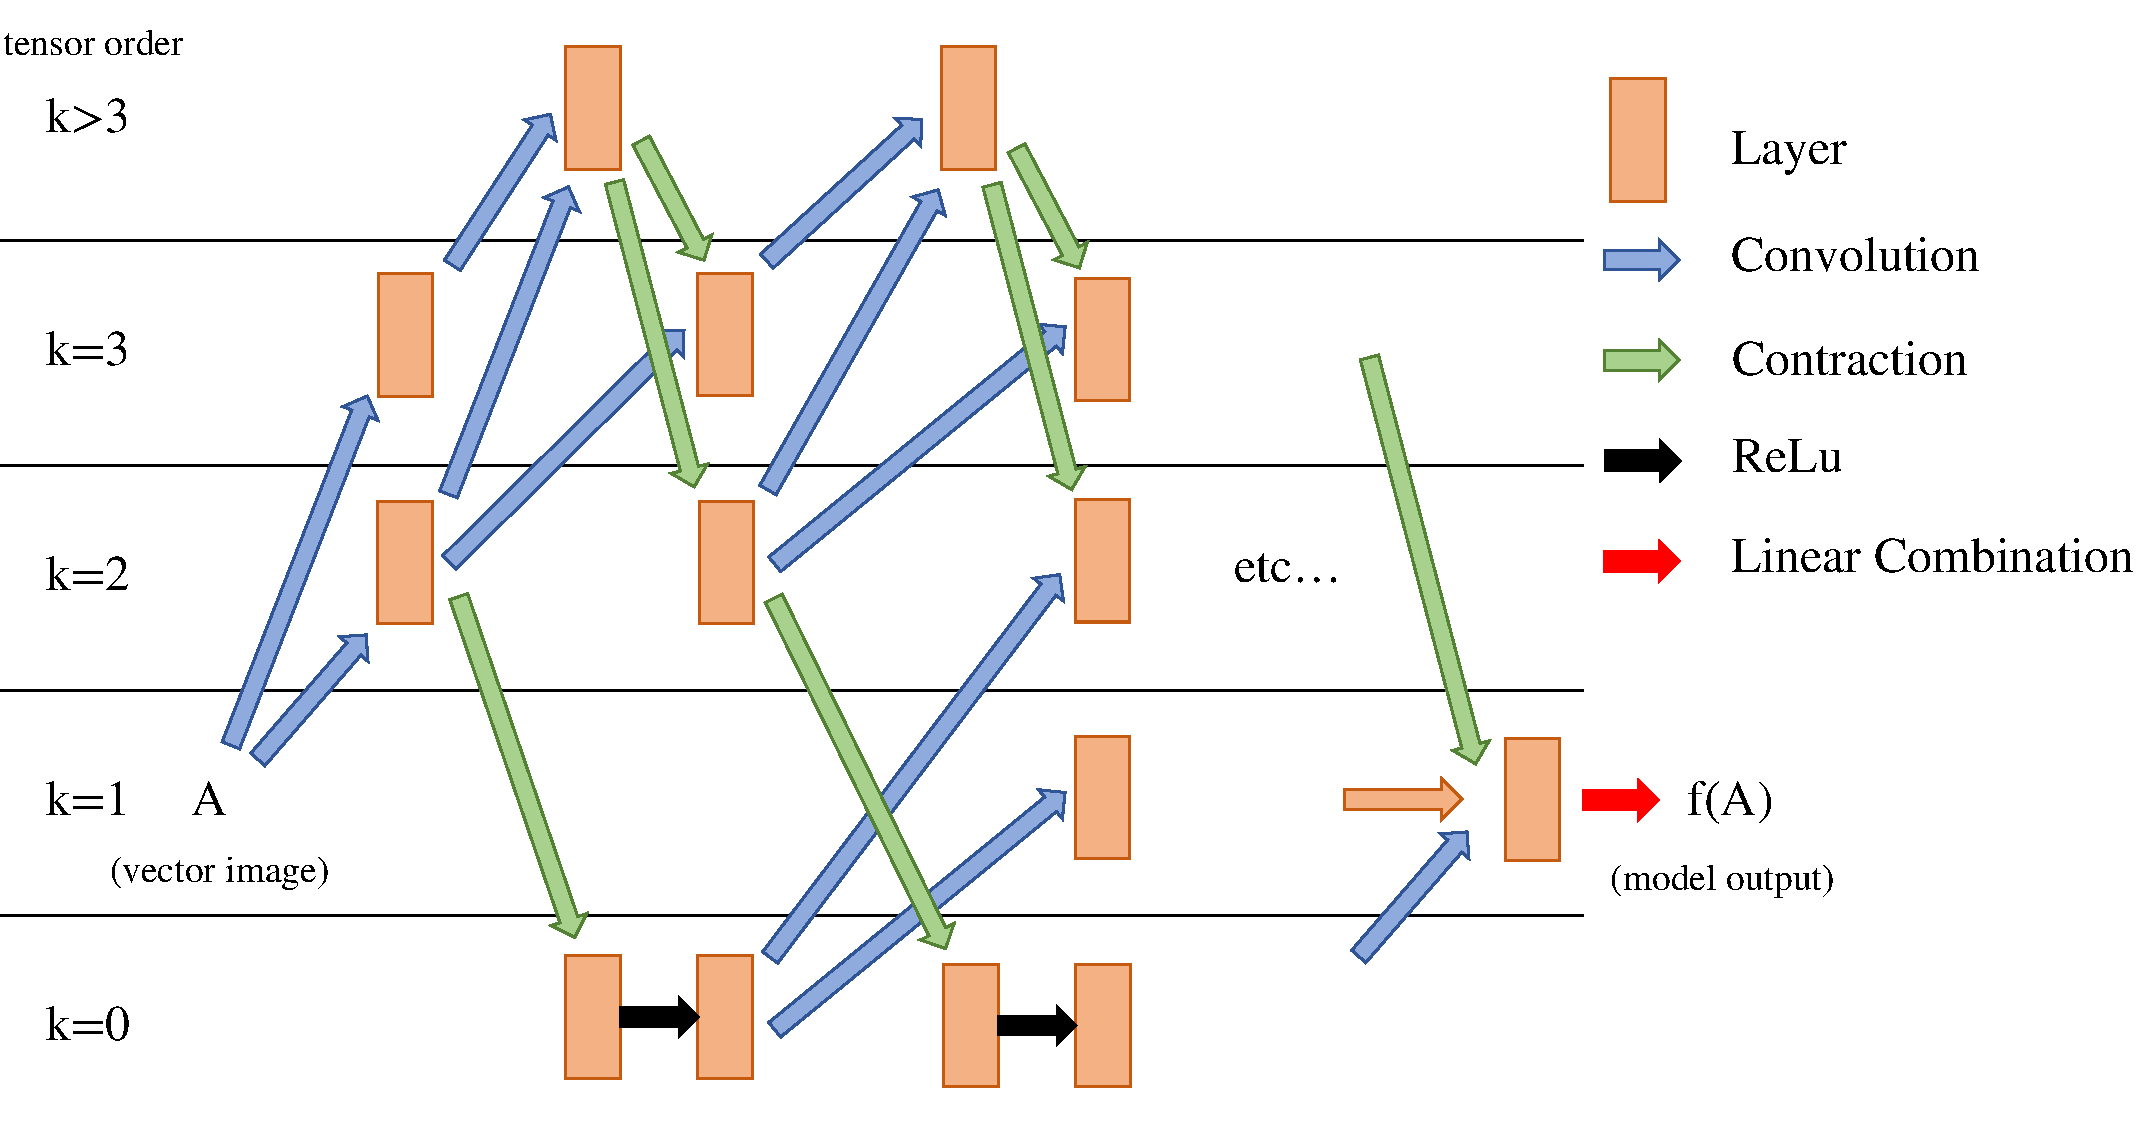
\includegraphics[width=0.75\textwidth]{architecture_diagram.pdf}\vspace{-0.15in}\end{center}
  \caption{One possible architecture for a GeometricImageNet \cite{gregory2023geometricimagenet} which maps a vector image to a vector image using convolution filters with tensor tensor filters and ReLu nonlinearities. Each layer is a block of multiple images that share tensor order. The blue arrows represent convolutions and raise the tensor order by 1 or 2. Contractions are applied when the tensor order goes above 3 to bring it down to 2 or 3, and when contracting to $k=0$ in order to apply the ReLu. This process continues until the final step where the only layer is order $k=1$, which is then combined using a parameterized linear combination. See \cite{gregory2023geometricimagenet} for details.}
  \label{fig:architecture}
\end{mdframed}\end{figure}

So far, we have only applied networks built from GeometricImageNet layers to small toy problems.
However, we conjecture that the current generations of emulators used in cosmology (for example \cite{chen2020learning}) and ocean science (for example \cite{bolton2019applications}), which are based on convolutional neural networks, will train with less training data and perform more accurate emulations when the CNN is replaced with the GeometricImageNet model of comparable depth and model complexity.

\section{\raggedright Strategies for symmetry-based adversarial attacks}\label{app:adversarial}
Each symmetry or conservation law in play in a physics problem leads to a vector for adversarial attack against an emulator for that problem.
For example, a simulation on a square grid obeys a rotation symmetry where the inputs can be rotated through 90 degrees and the outputs should end up so rotated.
One kind of adversarial attack against an emulator of that simulation is to find distortions of initial conditions that maximize the difference between the output and the de-rotated output from a rotated input.
That is, an adversarial attack created from a symmetry could involve searches for emulator inputs that maximally violate the symmetry.

Symmetries and conservation laws are more valuable as they become more local, and as more of the simulation fields are tracked.
For example, momentum conservation is a symmetry that applies to every subvolume of every simulation, provided that the simulation outputs are rich enough to track stress fields.
This is because the momentum conservation can be seen as a local equality between the rate of change of the local momentum density and the divergence of the local stress tensor field.
Thus some symmetries lead to very high dimensional predictions or predictions that apply to essentially every grid cell in a simulation at every time step.
When an emulator produces sufficient output, there might be very detailed attack strategies against that emulator.
Again, the attack would be to search for inputs such that there is a maximal violation of the local prediction from the conservation law.

The idea underlying this white paper is that we should define these kinds of attacks, implement them against real ocean-science and cosmology emulators, and develop adversarial training or mitigation strategies to improve future emulators.
Some examples of possible strategies follow.
This isn't in any sense an exhaustive list of what could be done.

Consider spaces $X$ and $Y$ and a group $G$ acting by representations $\phi$ and $\psi$ respectively. An emulator $f: X \to Y$  is equivariant (or covariant) with respect to the action of $G$ if
\begin{align}
    f(x) &= \psi(g)^{-1} f( \phi(g)\,x) ~ \forall g\in G, ~ x \in X, \label{eq.symmetry}
\end{align}
where $x$ is the input of the emulator, and $f(x)$ is the output of the emulator.
In non-trivial situations, the action of $g$ on $f(x)$ will be different from the action of $g$ on $x$, this why we consider different representations for $X$ and $Y$.
In principle, any violation of \eqref{eq.symmetry} indicates a problem with the emulator.

An adversarial attack customized for input $x$ and group element $g$ would be an optimization that makes a small adjustment $\xi$ to the input $x$ such that
\begin{align}
    \hat{\xi}(x,g;\epsilon) &\leftarrow \arg\max_{\xi} \left\{\|f(x+\xi) - \psi(g)^{-1} f(\phi(g)\,[x+\xi])\|\right\} ~\text{subject to}~\|\xi\|_\infty\leq\epsilon
\end{align}
where $\epsilon$ is a small perturbation amplitude. This specializes the standard notion of adversarial attacks to the group equivariant setting.  

Similarly, imagine that there is a conserved quantity---it could be precisely conserved or even only approximately conserved---that can be written as a function $H_X: X \to V$ of the emulator input $x$, and a function $H_Y: Y \to V$ of the emulator output $f(x)\in Y$ satisfying $H_X(x)= H_Y(f(x))$.
There is a similar kind of adversarial attack in this case that could look like
\begin{align}
    \hat{\xi}(x;\epsilon) &\leftarrow \arg\max_\xi \left\{\|H_X(x + \xi) - H_Y(f(x+\xi))\|\right\} ~\text{subject to}~\|\xi\| = \epsilon ~.
\end{align}
More detailed attacks are possible when conservation laws imply local relationships or invariants inside the output state $f(x)$.

We propose to design adversarial training schemes built from these (or other) forms of attacks in order to produce models that satisfy the symmetries and conservation laws in a robust way.
We conjecture that this will be more effective at enforcing symmetries and conservation laws than current standard data augmentation techniques. 
\end{appendices}\clearpage

\footnotesize % if you want the references to take up fewer pages
% \renewcommand\refname{References Cited} % if you want to change the name
\bibliographystyle{IEEEtran}
\bibliography{emulator}

\end{document}
